\documentclass[tikz,border=12pt]{standalone}
\usepackage{tikz}
\usepackage{amsmath,amssymb}
\usepackage{lmodern} % Latin Modern fonts for better rendering
\usepackage[T1]{fontenc}
\usepackage{microtype} % Better typography

\usetikzlibrary{arrows.meta,positioning,calc}

\tikzset{
    every node/.style={color=black, font=\sffamily\small},
    every math node/.style={font=\small},
    every path/.style={color=black},
    every circle/.style={draw=black},
    every rectangle/.style={draw=black}
}

\begin{document}
    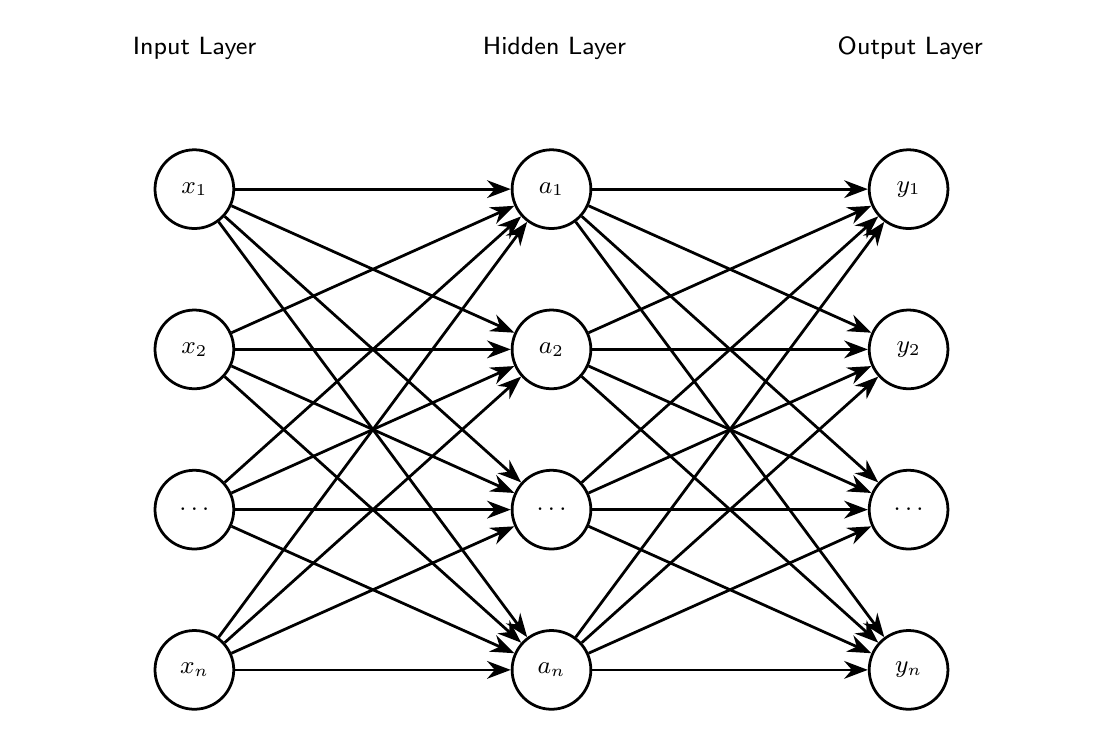
\begin{tikzpicture}[
        node distance=1cm,
        line width=1pt,
        >={Stealth[length=3mm]},
        neuron/.style={circle, draw, minimum size=1cm},
        layer/.style={circle, draw, minimum size=1cm},
        annot/.style={text width=4cm, align=center, anchor=north}
    ]


    % Nodes
    \node[neuron]                   (input1) {$x_1$};
    % Annotations aligned in one line at the top
    \node[annot, above=of input1]  (input layer)  {Input Layer};
    \node[annot, right=0.3cm of input layer] (hidden layer)  {Hidden Layer};
    \node[annot,  right=0.25cm of hidden layer] (output layer)  {Output Layer};
    \node[neuron, below=of input1]  (input2) {$x_2$};
    \node[neuron, below=of input2]  (input3) {$\ldots$};
    \node[neuron, below=of input3]  (input4) {$x_n$};

    % Hidden layer
    \node[layer, right=3.5cm of input1] (layer1) {$a_1$};
    \node[layer, below=of layer1] (layer2) {$a_2$};
    \node[layer, below=of layer2] (layer3) {$\ldots$};
    \node[layer, below=of layer3] (layer4) {$a_n$};

    \node[neuron, right=3.5cm of layer1] (output1) {$y_1$};
    \node[neuron, below=of output1] (output2) {$y_2$};
    \node[neuron, below=of output2] (output3) {$\ldots$};
    \node[neuron, below=of output3] (output4) {$y_n$};

    % Connections input -> hidden
    \foreach \i in {1,...,4}
        \foreach \j in {1,...,4}
            \draw[->] (input\i) -- (layer\j);

    \foreach \i in {1,...,4}
        \foreach \j in {1,...,4}
            \draw[->] (layer\i) -- (output\j);


    \end{tikzpicture}

\end{document}
